%%%%%%%%%%%%%%%%%%%%%%%%%%%%%%%%%%%%%%%%%%%%%%%%%%%%%%%%%%%%%%%%%%%%%%%%%%%
% This is LaTeX file for Homework Assignment 3
% Author: Shuo Yang
%%%%%%%%%%%%%%%%%%%%%%%%%%%%%%%%%%%%%%%%%%%%%%%%%%%%%%%%%%%%%%%%%%%%%%%%%%%

\documentclass[11pt]{article}
\usepackage{amsmath,amssymb,epsfig,graphics,hyperref,amsthm,mathtools}
\DeclarePairedDelimiter\ceil{\lceil}{\rceil}
\DeclarePairedDelimiter\floor{\lfloor}{\rfloor}

\hypersetup{colorlinks=true}

\setlength{\textwidth}{7in}
\setlength{\topmargin}{-0.575in}
\setlength{\textheight}{9.25in}
\setlength{\oddsidemargin}{-.25in}
\setlength{\evensidemargin}{-.25in}

\reversemarginpar
\setlength{\marginparsep}{-15mm}

\newcommand{\rmv}[1]{}
\newcommand{\bemph}[1]{{\bfseries\itshape#1}}
\newcommand{\N}{\mathbb{N}}
\newcommand{\Z}{\mathbb{Z}}
\newcommand{\imply}{\to}
\newcommand{\bic}{\leftrightarrow}

% Some user defined strings for the homework assignment
%
\def\CourseCode{CS545}
\def\AssignmentNo{3}
\def\DateHandedOut{Spring, 2015}
\def\DateDue{March 26}
\def\Author{Shuo Yang}

\begin{document}

\noindent

\CourseCode \hfill \DateHandedOut

\begin{center}
Homework Assignment \#\AssignmentNo\\
Due: \DateDue\\
Student: \Author\\
\end{center}

% A horizontal split line
\hrule\smallskip

% Enumerate through all questions.
\begin{enumerate}

\item % Problem 1
% Enumerate through all subquestions.
\begin{enumerate} % nested enumeration
\item Suppose we have 6 activities, for activity $i$, $s_i$ is the
  start time, $f_i$ is the finish time and $d_i$ is the duration. 
And we sort them in order of increasing duration:\\\\
\begin{tabular}{ l | l | l }
   & Points you get & 2 & 3 & 4 & 5 & 6\\ \hline
  $i$ & 1 & 2 & 3 & 4 & 5 & 6\\ \hline
\end{tabular}

The greedy procedure when the activities are considered in order of
increasing duration would be: 1) select activity 1 since it is the
local best; 2) select activity 2 since it is compatible with activity
1; 3) no other activities can be selected since they are not
compatible with either activity 1 or 2. So the procedure yields the
solution $\{1,2\}$, but the optimal solution should be
$\{3,4,1\}$. Therefore the greedy procedure is not correct.

\item With the same input, now let us sort them in order of increasing
  start-time:\\

\begin{tabular}{ l | l l l l l l }
  $i$ & 1 & 2 & 3 & 4 & 5 & 6\\ \hline
  $s_i$ & 0 & 1 & 3 & 4 & 4 & 8\\
  $f_i$ & 6 & 4 & 5 & 8 & 9 & 9\\
\end{tabular}

The greedy procedure when the activities are considered in order of
increasing duration is:

\textbf{Function} $GreedyActivitySelection(S, F, n)$\\
\-\hspace{3em} $A := \{1\}$ // activity with the earliest start time\\
\-\hspace{3em} $j := 1$ // indicates the activity with greatest start time in $A$\\
\-\hspace{3em} \textbf{for} $i := 2$ to $n$ \\
\-\hspace{5em} \textbf{if} $S[i] \geq F[j]$ \\
\-\hspace{7em} $A := A \cup \{i\}$ \\
\-\hspace{7em} $j := i$ \\
\-\hspace{3em} \textbf{return} $A$ \\

Running the above procedure with the same input yields the solution
$\{1,6\}$ which is certainly not an optimal solution. Therefore the
greedy procedure is not correct.

\item Consider the following 9 activities ordered by the number of
  overlaps which is denoted by $o_i$:\\

\begin{tabular}{ l | l l l l l l l l l }
  $i$ & 1 & 2 & 3 & 4 & 5 & 6 & 7 & 8 & 9\\ \hline
  $s_i$ & 4 & 0 & 7 & 1 & 2 & 3 & 5 & 6 & 6\\
  $f_i$ & 6 & 3 & 10 & 4 & 4 & 5 & 7 & 8 & 9\\
  $o_i$ & 2 & 2 & 2 & 3 & 3 & 3 & 3 & 3 & 3\\
\end{tabular}

When considering the order of increasing number of overlaps, the
greedy procedure would first pick activity 1, then pick activity 2,
and finally pick activity 3.
Thus the solution derived by the greedy procedure is $\{1,2,3\}$, but the
optimal solution should be $\{2,6,7,3\}$. Therefore the
greedy procedure is not correct.

\end{enumerate}

\item % problem 2
Label $n$ gas stations as $g_1,g_2,\cdots,g_n$ and let $d_i$ be the
distance between gas stations $g_i$ and $g_{i+1}$, specially, $d_0$
denotes the distance between $g_1$ and city $A$, and $d_{n}$ denotes
the distance between city $B$ and $g_n$. Let $D$ be the total distance
between city $A$ and $B$, where $D=\sum_{i=0}^{n} d_i$.

\underline{\textbf{Greedy algorithm}}

The greedy strategy is to refuel at the gas station whose distance
from the current stop is closest to $m$ but less than $m$.\\

\textbf{Function} $GreedyTripRefuel()$\\
\-\hspace{3em} $A := \emptyset$ // the set of refueling stops\\
\-\hspace{3em} $i := 0$ // indicates the farthest gas station one can
make.\\
\-\hspace{3em} $T_1 := 0$ // distance traveled before making a
refuel\\
\-\hspace{3em} $T_2 := 0$ // total distance traveled \\
\-\hspace{3em} \textbf{while} $T_2 < D$ \\
\-\hspace{5em} \textbf{if} $(T_2 - T_1) \leq m$ \\
\-\hspace{7em} $T_2 := T_2 + d_i$ \\
\-\hspace{7em} $i := i + 1$ \\
\-\hspace{5em} \textbf{else} \\
\-\hspace{7em} $i := i - 1$ // cannot make it to station $g_i$, so
must refuel at station $g_{i-1}$\\ 
\-\hspace{7em} $A := A \cup \{g_i\}$ \\
\-\hspace{7em} $T_2 := T_2 - d_i$ \\
\-\hspace{7em} $T_1 := T_2$ \\
\-\hspace{3em} \textbf{return} $A$ \\

The algorithm runs in $O(n)$ time since there are at most $n$ gas
stations along the way.

\underline{\textbf{Correctness}}

\textbf{Lemma:} Suppose $A$ is a subset of an optimal solution where
the latest refuel stop is station $g_k$. Let $g_i$ be the gas station
after $g_k$ whose distance from $g_k$ is closest to $m$ but less than
$m$. Then $A \cup \{g_i\}$ is also a subset of an optimal solution.

\begin{proof}
  Since $A$ is a subset of an optimal solution, let $A^*$ be an
  optimal solution with $A \subseteq A^*$. Let $g_j$ be the gas station in
  $A^* - A$ that is next to $g_k$. We have two cases:
  \begin{itemize}
  \item case-1: $i = j$. Then $A \cup \{g_i\} \subseteq A^*$, the lemma
    holds. 
  \item case-2: $i \neq j$. Since the distance from $g_k$ to $g_i$ is
    closest to $m$ but less than $m$, this distance must be greater
    than the distance from $g_k$ to $g_j$. Thus we can replace $g_j$
    with $g_i$ and still yields an optimal solution since $g_i$ is
    closer to the future stops than $g_j$.
  \end{itemize}
\end{proof}

\textbf{Theorem:} $GreedyTripRefuel()$ finds an optimal solution.

\begin{proof}
  Initially, $A$ is an empty set, which is a subset of an
  optimal solution and $g_k$ in this case would be city $A$. By the
  lemma, $A \cup g_i$ is a subset of an optimal solution where $g_i$
  is the gas station whose distance from city $A$ is closest to $m$
  but less than $m$. 

  By induction on the number of iterations, when the function
  terminates, $A$ is a subset of an optimal solution. 

  Since from the starting point, the greedy algorithm makes the least
  possible stops, there is no better solution with fewer stops than
  the one produced by the greedy algorithm. Therefore $A$ is optimal.
\end{proof}

\item % problem 3
\begin{enumerate}
\item % part-a
\underline{\textbf{Greedy algorithm}}

Let the set of $n$ tasks be $\{a_i | 1 \leq i \leq n\}$. The greedy
strategy is to schedule the shortest task first.
\begin{enumerate}
\item Merge sort the $n$ tasks in the order of increasing execution time
such that $t_1 \leq t_2 \leq \cdots \leq t_n$.
\item Schedule the tasks in the order of $\{a_1,a_2,\cdots,a_n\}$.
\end{enumerate}

Step (a) takes $O(n\log n)$ time and step (b) takes $O(n)$ time, thus
the overall runtime is $O(n\log n)$.

\underline{\textbf{Correctness}}

First, we define containment relationship.\\
We define $\{a_1,a_2,\cdots,a_m\}$ as a schedule sequence such that $a_i$
is scheduled after $a_{i-1}$ where $1 < i \leq m$.
For a schedule sequence $\{a_1,a_2,\cdots,a_n\}$, we define
$\{a_1,a_2,\cdots,a_k\}$ as a prefix-subsequence of it where $k \leq n$.

\textbf{Lemma:} Suppose $A$ is a prefix-subsequence of an optimal schedule
sequence. Let $a_i$ be the task that has the shortest execution time
among those tasks that are not in $A$. Let $A'$ be the
prefix-subsequence by appending $a_i$ to the end of $A$.
Then $A'$ is also a prefix-subsequence of an optimal schedule sequence.

\begin{proof}
  Since $A$ is a prefix-subsequence of an optimal schedule sequence,
  let $A^*$ be the optimal schedule sequence that contains $A$ as a
  prefix-subsequence. Let $a_i$ be the task that has the shortest
  execution time among those tasks in $A^*-A$. By appending $a_i$ to
  the end of the $A$, we get another prefix-subsequence $A'$. There
  are two cases:
  \begin{enumerate}
  \item $A'$ is a prefix-subsequence of $A^*$, the lemma holds.
  \item $A'$ is not a prefix-subsequence of $A^*$, Let $a_j$ be the
    task that appears first in the subsequence $A^*-A$. In
    this case we must have: $t_i = t_j$. We prove this by 
    contradiction:\\
    Suppose $t_i \neq t_j$, since $a_i$ is the task with the shortest
    execution time in $A^*-A$, we must have: $t_j > t_i$. Let the last
    task in $A$ be $a_m$. Without loss of generality, assume $A^*-A$
    is ordered as
    $a_j,a_{x_1},\cdots,a_{x_s},a_i,a_{y_1},\cdots,a_{y_r}$ such that
    there are $s$ tasks scheduled after $a_j$ and before $a_i$, and
    there are $r$ tasks scheduled after $a_i$. Let $c_{x_k}$ denotes
    the completion time for the tasks scheduled in between $a_j$ and
    $a_i$, and let $c_{y_k}$ the completion time for the tasks
    scheduled after $a_i$. We have:
    \begin{align}
      c_j &= c_m + t_j\\
      c_{x_k} &= c_j + \sum_{1 \leq i \leq k}^{k \leq s}t_{x_i}\\
      c_i &= c_j + \sum_{1 \leq i \leq s}t_{x_i} + t_i\\
      c_{y_k} &= c_i + \sum_{1 \leq i \leq k}^{k \leq r}t_{y_i}
    \end{align}

    Now suppose we exchange the positions of $a_i$ and $a_j$ to
    produce another subsequence $(A^*-A)'$\\
    $a_i,a_{x_1},\cdots,a_{x_s},a_j,a_{y_1},\cdots,a_{y_r}$ and
    together with $A$, this produces another schedule sequence $A^{*'}$. In this
    case, let $c_j'$ be the completion time for $a_j$, $c_i'$ be the
    completion time for $a_i$, $c_{x_k}'$ be
    the completion time for the tasks scheduled in between $a_j$ and
    $a_i$, and let $c_{y_k}'$ be the completion time for the tasks
    scheduled after $a_j$. We have:
    \begin{align}
      c_i' &= c_m + t_i\\
      c_{x_k}' &= c_i' + \sum_{1 \leq i \leq k}^{k \leq s}t_{x_i}\\
      c_j' &= c_i' + \sum_{1 \leq i \leq s}t_{x_i} + t_j\\
      c_{y_k}' &= c_j' + \sum_{1 \leq i \leq k}^{k \leq r}t_{y_i}
    \end{align}
    
    Now we compare completion times for the two subsequences:
    \begin{align}
      c_j - c_i' &= (c_m + t_j) - (c_m + t_i)\\
      &= t_j - t_i\\
      &> 0\\
      c_{x_k} - c_{x_k}' &= (c_j + \sum_{1 \leq i \leq k}^{k \leq
        s}t_{x_i}) - (c_i' + \sum_{1 \leq i \leq k}^{k \leq
        s}t_{x_i})\\ 
      &= c_j - c_i'\\
      &> 0\\
      c_i - c_j' &= (c_j + \sum_{1 \leq i \leq s}t_{x_i} + t_i) -
      (c_i' + \sum_{1 \leq i \leq s}t_{x_i} + t_j)\\ 
      &= c_j - c_i' + t_i - t_j\\
      &= t_j - t_i' + t_i - t_j\\
      &= 0\\
      c_{y_k} - c_{y_k}' &= (c_i + \sum_{1 \leq i \leq k}^{k \leq
        r}t_{y_i}) - (c_j' + \sum_{1 \leq i \leq k}^{k \leq
        r}t_{y_i})\\
      &= c_i - c_j'\\
      &= 0
    \end{align}
    Therefore, the sum of the completion time for $A^*-A$ is
    absolutely greater than the sum of the completion time for
    $(A^*-A)'$. So the average completion time of $A^*$ must be greater
    than that of $A^{*'}$, we have found a better solution than
    $A^*$. This contradicts the fact that $A^*$ is an optimal
    solution. Thus we must have $t_i = t_j$. 

    So we can get another optimal schedule sequence by exchanging the order of
    $a_i$ and $a_j$ because since $t_i = t_j$, the exchange will not
    affect the overall average completion time. And this new optimal
    schedule sequence has $A'$ as a prefix-subsequence. The lemma
    still holds.
  \end{enumerate}
\end{proof}

\textbf{Theorem:} The greedy algorithm finds an optimal schedule sequence.

\begin{proof}
  Initially, $A$ is a empty sequence, which is always a
  prefix-subsequence of any schedule sequence. Suppose all $n$ tasks
  $a_1,a_2,\cdots,a_n$ have been sorted in the order of increasing
  execution time. By the lemma, $\{a_1\}$ is a prefix-subsequence of
  an optimal schedule sequence. 
  
  By induction on the number of iterations, when the algorithm
  terminates, $A$ is still a prefix-subsequence of an optimal schedule
  sequence. And when the algorithm terminates, $A$ would contain all
  $n$ tasks, no other schedule sequence can properly contain $A$, thus
  $A$ is the optimal schedule sequence.
\end{proof}

\item % part-b

\underline{\textbf{Algorithm}}

The algorithm will use the shortest-remaining-time policy to find an
optimal schedule. It uses a min-heap to organize the released but not
completed tasks where heap ordering is based on their remaining
execution times. A scheduling decision is made when a task is
completed or when a new task is released.\\

Assume that the heap has the following operations:
\begin{itemize}
\item $heap.insert(a,r)$: insert task $a$ with the remaining time $r$.
\item $heap.pop()$: remove the task $a$ with the smallest remaining
  time $r$ and return the pair $(a,r)$.
\item $heap.findmin()$: find the task $a$ with the smallest remaining
  time $r$ and return the pair $(a,r)$.
\item $heap.notempty()$: return true if the heap is not empty,
  otherwise return false.\\
\end{itemize}

Let $A$ be the set of $n$ tasks: $\{a_i | 1 \leq i \leq n\}$, $T$ be
the set of execution times: $\{t_i | 1 \leq i \leq n\}$, and $R$ be the 
set of release times: $\{r_i | 1 \leq i \leq n\}$. The scheduling
algorithm is implemented as
follows:\\\\\\\\\\\\\\\\\\\\\\\\\\\\\\\\\\\\\\\\\\\\\\\\\\\\

\textbf{Function} $SRTFschedule(heap, A, R, T, r)$\\
\-\hspace{2em} sort tasks in the order of increasing releasing time
using quick sort\\
\-\hspace{2em} $S := \emptyset$ // set of scheduled tasks\\
\-\hspace{2em} $i := 1$ \\
\-\hspace{2em} $minr_1 := r_i$ // start time for the next scheduled task\\
\-\hspace{2em} $heap.insert(a_i,t_i)$ \\
\-\hspace{2em} \textbf{while} $r_{i+1} == r_i$\\
\-\hspace{4em} $i := i + 1$ \\
\-\hspace{4em} $heap.insert(a_i,t_i)$ \\
\-\hspace{2em} $i := i + 1$ \\
\-\hspace{2em} \textbf{while} $i \leq n$\\
\-\hspace{4em} $minr_2 := r_i$ // next release time\\
\-\hspace{4em} $(a,r) := heap.pop()$\\
\-\hspace{4em} $S := S \cup \{a\}$ // schedule task $a$\\
\-\hspace{4em} \textbf{if} $minr_2 - minr_1 \geq r$ //task $a$ can
finish before the next batch of released tasks\\
\-\hspace{6em} $minr_1 := minr_1 + r$ // update the start time for the
next scheduled task\\
\-\hspace{6em} $(a,r) = heap.pop()$ // schedule the next task on heap
before next batch of release \\
\-\hspace{6em} $S := S \cup \{a\}$\\
\-\hspace{4em} \textbf{else} // task $a$ runs for $(minr_2-minr_1)$
time, then the next batch of release comes\\
\-\hspace{6em} $heap.insert(a_i,t_i)$ \\
\-\hspace{6em} \textbf{while} $r_{i+1} == r_i$\\
\-\hspace{8em} $i := i + 1$ \\
\-\hspace{8em} $heap.insert(a_i,t_i)$ \\
\-\hspace{6em} $i := i + 1$ \\
\-\hspace{6em} $(a',r') := heap.findmin()$\\
\-\hspace{6em} $r := r - (minr_2 - minr_1)$ // update the remaining
time for task $a$\\
\-\hspace{6em} $minr_1 = minr_2$ // update $minr_1$\\
\-\hspace{6em} \textbf{if} $r' \geq r$ // continue to run task $a$\\
\-\hspace{8em} \textbf{continue}\\
\-\hspace{6em} \textbf{else} // current running task $a$ is preempted\\
\-\hspace{8em} $heap.insert(a,r)$ // put task $a$ back to the heap\\
\-\hspace{8em} $(a,r) := heap.pop()$ // schedule the task with the
smallest remaining time\\
\-\hspace{8em} $S := S \cup \{a\}$\\\\
\-\hspace{2em} \textbf{while} heap.notempty() // no more tasks to
release\\
\-\hspace{4em} $(a,r) := heap.pop()$\\
\-\hspace{4em} $S := S \cup \{a\}$\\

\underline{\textbf{Runtime}}

Quick sort takes $O(n\log n)$ time;\\
$heap.insert()$ and $heap.pop()$ take $O(\log n)$ time;\\
$heap.findmain()$ takes $O(1)$ time;\\
The first outer-most \textbf{while} loop takes $O(n\log n)$ time;\\
The second outer-most \textbf{while} loop takes $O(n\log n)$ time;
note that although there is another \textbf{while} loop inside the
outer-loop, this inner-loop will increment the value of $i$
which decrement the number of iterations of the outer-loop, thus the
amortized cost for each iteration of outer-loop is still $O(\log
n)$.\\
The third outer-most \textbf{while} loop also takes $O(n\log n)$ time;\\
Thus the total run time of the algorithm is $O(n\log n)$.

\underline{\textbf{Correctness}}

\textbf{Theorem:} Shortest-remaining-time-first schedule is optimal.

\begin{proof}
  Prove by contradiction.\\
  Assume that Shortest-remaining-time-first schedule is not
  optimal, then there exists an optimal schedule $S$ that does not use
  shortest-remaining-time-first policy.\\
  Suppose at time $t$, instead of scheduling task $i$ with the
  shortest-remaining-time at the time being, $S$ schedules task $k$
  with longer remaining-time. Let $R_i$ and $R_j$ be the remaining
  time for tasks $i$ and $j$, and $C_i$ and $C_j$ be the completion
  time for tasks $i$ and $j$. We have: $R_i < R_j$. In total, $R_i + 
  R_j$ is spent on tasks $i$ and $j$ after time $t$. We assume that
  $C_i < C_j$. 

  We can get another schedule $S'$ by interchanging schedule sequence
  of tasks $i$ and $j$:
  \begin{enumerate}
  \item devote the first $R_i$ units of time that were distributed to
    either task $i$ or $j$ after $t$ completely to task $i$ until its
    completion. 
  \item devote the remaining $R_j$ units of time for task $j$ since
    task $i$ has completed.
  \end{enumerate}
  The two schedules are shown in the figure below.\\
  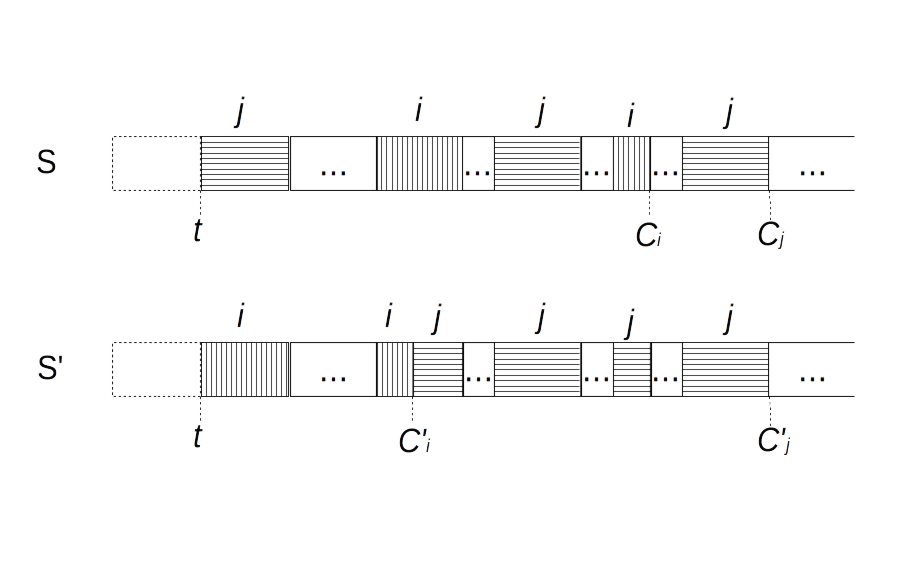
\includegraphics[width=12cm,height=8cm]{../imgs/SRTF-schedule.png}

  Let $C_i'$ and $C_j'$ be the completion time for tasks $i$ and $j$
  in the new schedule $S'$.

  By doing this interchanging, we get a better solution, because:
  \begin{align}
    C_i &> C_i'\\
    C_j &= C_j'
  \end{align}
  Since in the new schedule, other tasks other than task $i$ have the
  same completion time as before, thus the total sum of completion of
  the new schedule $S'$ is less than that of $S$. This contradicts the
  fact that $S'$ is optimal. Thus shortest-remaining-time-first
  schedule is optimal. 
\end{proof}

\end{enumerate}

\item % problem 4
\begin{enumerate}
\item \underline{\textbf{Greedy algorithm}}

The greedy strategy is to always choose the largest denomination that
is not greater than the remaining amount.

The function $GreedyCoinChange(n)$ implements this strategy.\\\\\\

\textbf{Function} $GreedyCoinChange(n)$\\
\-\hspace{3em} $A := \emptyset$ // the set of choose coins \\
\-\hspace{3em} $denominations := \{25,10,5,1\}$ // set of
available denominations \\
\-\hspace{3em} \textbf{while} $n > 0$\\
\-\hspace{5em} $x := $ the largest value in $denominations$ that is
$\leq n$ \\
\-\hspace{5em} $A := A \cup \{x\}$ // pick $x$\\
\-\hspace{5em} $n := n - x$\\
\-\hspace{3em} \textbf{return} $A$\\

The runtime of the algorithm is $O(n)$.

\underline{\textbf{Correctness}}

First, we make the following claims:
\begin{itemize}
\item Claim-1: There cannot be more than 4 pennies in an optimal
  solution because 5 pennies can be replaced by 1 nickle which yields
  a better solution with 4 coins less.
\item Claim-2: There cannot be more than 1 nickle in an optimal
  solution because 2 nickles can be replaced by 1 dime which yields
  a better solution with 1 coin less.
\item Claim-3: There cannot be more than 2 dimes in an optimal
  solution because 3 dimes can be replaced by 1 quarter and 1 nickle
  which yield a better solution with 1 coin less.
\item Claim-4: There cannot be 2 dimes and 1 nickle both in an optimal
  solution because 2 dimes and 1 nickle can be replaced by 1 quarter
  which yield a better solution with 2 coins less.
\end{itemize}

\textbf{Lemma:} Suppose $A$ is a subset of an optimal solution $A^*$.
Let $m$ be the amount of the remaining cents, that is, total cents in $A^*-A$.
Let $x$ be the largest value among $\{25,10,5,1\}$ that is not greater
than $m$. Then $A' = A \cup \{x\}$ is also a subset of an optimal solution.

\begin{proof}
  We prove by cases. There are total 4 cases.
\begin{itemize}
\item Case-1: x = 25.\\
  In this case, we have $m \geq 25$. If $x \in A^*-A$, the lemma
  holds. If $x \notin A^*-A$, then $A^*-A$ cannot contain quarters. We
  have two sub-cases: 1) $25 \leq m < 30$, then the best possible solution is to
  pick 2 dimes and 1 nickle, and $m-25$ pennies. But this violates the
  \emph{Claim-4}; 2) $m \geq 30$, then the best possible solution must contain at
  least 3 dimes, but this violates the \emph{Claim-3}. Since in both
  sub-cases, the best possible solutions violate some claims, we know
  that they must not be subset of an optimal solution. Therefore $x$
  must be in $A^*-A$, the lemma holds.
\item Case-2: x = 10.\\
  In this case, we have $10 \leq m < 25$. If $x \in A^*-A$, the lemma
  holds. If $x \notin A^*-A$, then $A^*-A$ cannot contain quarters and
  dimes. The best possible solution is to pick at least 2 nickles, but
  this violates the \emph{Claim-2}. So $x$ must be in $A^*-A$, the
  lemma holds. 
\item Case-3: x = 5.\\
  In this case, we have $5 \leq m < 10$. If $x \in A^*-A$, the lemma
  holds. If $x \notin A^*-A$, then $A^*-A$ cannot contain quarters,
  dimes and nickles. The best possible solution is to pick $m$
  pennies, but this violates the \emph{Claim-1}. So $x$ must be in
  $A^*-A$, the lemma holds.
\item Case-4: x = 1.\\
  In this case, we have $1 \leq m < 5$ and $x$ must be in
  $A^*-A$ because pennies are the only choices, thus the lemma holds.
\end{itemize}
Since for all 4 cases, the lemma holds, it must be true.
\end{proof}

\underline{\textbf{Theorem:}} Greedy algorithm $GreedyCoinChange$
finds an optimal solution.

\begin{proof}
  Initially, $A$ is an empty set which is always a subset of any
  optimal solutions.By the lemma, $\{x\}$ is a subset of an optimal
  solution where $x$ is the largest denomination that is not greater
  than $n$. By induction on the number of iterations, when 
  the algorithm terminates, $A$ is still a subset of an optimal
  solution. When the algorithm terminates, $A$ would contain coins
  with the total amount equals $n$ and satisfy the 4 claims, thus no
  other solutions can properly contain $A$, thus $A$ is optimal.
\end{proof}

\item % part-b
  \begin{proof}
    prove by giving an counter example. Suppose the denomination system
    is the set: $\{1,3,4\}$ and $n=6$. The greedy algorithm
    $GreedyCoinChange$ yields the solution $\{4,1,1\}$. But the optimal
    solution is $\{3,3\}$. This proves that greedy algorithm from Part
    (a) does not make optimal change for all systems of coins.
  \end{proof}

\item % part-c
  \underline{\textbf{Lemma:}} There cannot be more than $(a-1)$
  coins with the value $a^i$ in an optimal solution where $0
  \leq i < k$.

  \begin{proof}
    Prove by contradiction. Suppose there is an optimal solution that
    contains more than $(a-1)$ coins of the value $a^i$ for
    some $i$ where $0 \leq i < k$. But $a$ coins of the value $a^i$
    can be replaced with 1 coin with the value of $a^{i+1}$. This
    yields a better solution with $a-1$ coins less since $a > 1$. This
    is a contradiction. Therefore the lemma must always hold.
  \end{proof}

  \underline{\textbf{Theorem:}} The greedy algorithm in part-a makes optimal
  change for the system of coins with denominations
  $\{a^0,a^1,\cdots,a^k\}$ where $a>1$ and $k \geq 1$.

  \begin{proof}
    Prove by contradiction.\\
    Let $A$ be the solution found by the greedy
    algorithm. Suppose $A$ is not optimal, then let $A'$ be an
    optimal solution. Define $C = \{c_i | 0 \leq i \leq k\}$ as the set
    of coin counts for $A$ where $c_i$ is the number of coins with the
    value of $a^i$ in $A$. And define $C' = \{c_i' | 0 \leq i \leq k\}$ as the set
    of coin counts for $A'$ where $c_i'$ is the number of coins with the
    value of $a^i$ in $A'$. 

    Let $j$ be the first highest index for which $c_j \neq c_j'$. Then
    we must have: $c_j > c_j'$ because our algorithm makes greedy
    choices locally and picks as much $a^j$ as possible and this is
    the first value on which they disagree. Also $j > 0$ because if
    only $c_0$ and $c_0'$ are different, then the total amount in $A$
    and $A'$ would be different. 

    Since $c_j > c_j'$ and $c_j' \geq 0$, the partial amount
    $B=\sum_{i=0}^{j-1} c_i' a^i$ in $A'$ must satisfy the condition
    that $B \geq a^j$.

    Also, by the lemma, the largest possible value for the partial
    amount $B$ is:
    \begin{align}
      \sum_{i=0}^{j-1} c_i' a^i &= (a-1)a^0 + (a-1)a^1 + \cdots +
      (a-1)a^{j-1}\\
      &= (a-1)\sum_{i=0}^{j-1} a^i\\
      &= (a-1)\frac{1-a^j}{1-a}\\
      &= a^j - 1\\
      &< a^j
    \end{align}

    This contradicts the fact that $B \geq a^j$. Thus $A$ must be an
    optimal solution.    
  \end{proof}

\item % part-d

  \underline{\textbf{Recursive structure of an optimal change}}

  Give a set of denomination $D = \{d_1,d_2,\cdots,d_k\}$ where $d_1 =
  1$ and an amount of cents $n$, an optimal change must start with one
  of coins in $D$, say it is 
  $d_i$ where $1 \leq i \leq k$. Then the optimal change must be $1+$
  (optimal change for $n-d_i$).

  \underline{\textbf{Recurrence equation}}

  Define $C(i)$ be the optimal number of changes made for amount of $i$
  cents. The goal value is $C(n)$.
  \begin{equation}
    C(i) := \begin{cases}
      \min\limits_{1 \leq j \leq k}(C(i-d_j)) + 1 \-\hspace{2em} i > 0\\
      0 \-\hspace{10.5em} i = 0\\
      \infty \-\hspace{10em} i < 0
    \end{cases}
  \end{equation}

  \underline{\textbf{Evaluate the recurrence equation}}

  We fill the table up from $C(0)$ until $C(n)$.

  The size of table is $O(n)$ and to fill each cell, we need $O(k)$
  comparison, so the total run time of filling the table is $O(kn)$.

  \underline{\textbf{Recover the optimal solution}}

  For the optimal number of coins, we simply look up the value of
  $C(n)$. 

  For the number of each denomination in the optimal solution, we can
  trace back to see how many coins are needed to make change for
  $(n-d_i)$ cents for each $i$ where $1 \leq i \leq k$, and choose the
  smallest number. Repeat this process until the remaining amount
  is $\leq$ 0.

\end{enumerate}

\end{enumerate}
\end{document}
